\subsubsection{Norme}
\subsubsubsection{Classificazione dei requisiti}
Gli \rAs hanno il compito di elencare una lista di requisiti  emersi durante lo studio e l'analisi del capitolato scelto ed eventualmente in seguito a degli incontri con il \gloxy{Proponente}.
I requisiti prodotti devono essere classificati per tipo e per importanza secondo la seguente codifica:
\begin{center}
R[Tipo][Importanza][Codice]
\end{center}
\vspace{0.2in}
\begin{itemize}
\item \textbf{Tipo}:  può assumere solo uno tra i seguenti valori:
\begin{itemize}
\item \textit{F}: Funzionale;
\item \textit{Q}: Qualità;
\item \textit{P}: Prestazionale;
\item \textit{V}: Vincolo.
\end{itemize}
\item \textbf{Importanza}: può assumere solo uno tra i seguenti valori:
\begin{itemize}
\item \textit{O}: Obbligatorio;
\item \textit{D}: Desiderabile;
\item \textit{F}: Facoltativo.
\end{itemize}
\item \textbf{Codice}: è il codice gerarchico, unico per ogni requisito, che viene espresso in forma numerica (esempio: 1.1.1).
\end{itemize}
Vengono inoltre specificati per ogni requisito:
\begin{itemize}
\item \textbf{Descrizione}: deve risultare sintetica, completa ed il meno ambigua possibile;
\item \textbf{Fonte}: deve risultare una o più tra le seguenti:
\begin{itemize}
\item \textit{Capitolato}: il requisito deriva direttamente dal capitolato;
\item \textit{Verbale}: il requisito è stato aggiunto in seguito ad un incontro con il \gloxy{Proponente} e verbalizzato;
\item \textit{Interno}: il requisito è derivato da considerazioni interne derivanti dall'applicazione di standard di qualità;
\item \textit{Caso d'uso}: il requisito è derivato da uno o più casi d'uso.
\end{itemize}
\end{itemize}
\subsubsubsection{Classificazione dei casi d'uso}
I casi d'uso prodotti devono essere descritti usando il seguente formato:
\begin{center}
UC[Codice padre].[Codice di livello]
\end{center}
\begin{itemize}
\item \textbf{Codice del padre}: codice del caso d'uso padre, se non è possibile individuare un caso d'uso padre, è da omettere;
\item \textbf{Codice di livello}: codice progressivo che identifica i casi d'uso figli.
\end{itemize}
Per ogni caso d'uso devono inoltre essere specificati:
\begin{itemize}
\item \textbf{Nome}: definizione del caso d'uso;
\item \textbf{Attori}: attori coinvolti nel caso d'uso;
\item \textbf{Descrizione}: chiara, completa e sintetica del caso d'uso;
\item \textbf{Precondizione}: condizione che deve essere vera al momento dell'esecuzione del caso d'uso;
\item \textbf{Postcondizione}: condizione che deve essere vera alla fine dell'esecuzione del caso d'uso;
\item \textbf{Scenario principale}: spiegazione composta dal flusso dei casi d'uso figli;
\item \textbf{Scenari Alternativi}: spiegazione composta dai casi d'uso non appartenenti al flusso principale;
\item \textbf{Estensioni}: spiegazione di tutte le estensioni, se presenti;
\item \textbf{Inclusioni}: spiegazione di tutte le inclusioni, se presenti;
\item \textbf{Generalizzazioni}: spiegazione di tutte le generalizzazioni, se presenti.
\end{itemize}
\subsubsubsection{Norme progettuali}\label{normeProgettuali}
\subsubsubsubsection{Denominazione di entità e relazioni}\label{sdeer}
Tutti i package, le classi, i metodi e gli attributi devono essere denominati in modo chiaro. Il nome deve avere una lunghezza che non ne pregiudichi chiarezza e leggibilità. Le abbreviazioni ai nomi degli elementi sono ammesse soltanto se risultano immediatamente comprensibili, contestualizzate e non devono causare ambiguità. Inoltre è preferibile utilizzare sostantivi per i nomi delle entità e verbi per le relazioni.
\subsubsubsubsection{Notazioni per la progettazione architetturale}
Poiché nel linguaggio \gloxy{JavaScript} le funzioni sono costrutti \gloxy{high-order} in aggiunta al formalismo \gloxy{UML} 2.0 è stata definita una notazione apposita per rappresentare il tipo di dato funzione: \texttt{function(<parameters>)}. Questa notazione rappresenta quindi il tipo funzione che richiede i parametri \texttt{<parameters>}.\\
%Inizio parte nuova
Durante la descrizione delle componenti viene spesso utilizzata la notazione ``\textit{oggetto contenente le informazioni riguardo ... organizzate come coppie chiave/valore}'' per indicare un oggetto \gloxy{JavaScript} che ha come campi dati le varie chiavi e ognuno di questi campi ha come valore il dato associato alla chiave. \\
Ad esempio ``\textit{un oggetto contenente le informazioni riguardanti i \gloxy{percorsi} presenti all'interno di un \gloxy{progetto}, organizzate come coppie chiave/valore, usando come chiave l'id del \gloxy{percorso} e come valore il nome}'' individua un oggetto che ha come campi dati tutti gli \texttt{id} dei vari \gloxy{percorsi di presentazione} e come valore del campo è assegnato il nome del \gloxy{percorso} di presentazione.
%fine parte nuova
Per facilitare la comprensione dei diagrammi \gloxy{UML} si è scelto di utilizzare il colore arancione per evidenziare le \gloxy{librerie} esterne inoltre, quando vengono presentati i diagrammi dei package, vengono mostrate le classi prive dei campi dati e dei metodi.\\
Questa scelta è stata fatta per evitare di creare diagrammi troppo grandi che sarebbero risultati illeggibili.
I diagrammi completi di ogni classe saranno quindi presenti solo vicino alle relative descrizioni.
\subsubsubsubsection{Notazioni per la progettazione di dettaglio}
\subsubsubsubsubsection{Notazioni per il \gloxy{Front-End}}\label{std_angular}
\subsubsubsubsubsubsection{\gloxy{Controller} e \$scope}\label{notazioneControllersAngularJS}
Nella definizione dei vari controllers dell'applicazione gli oggetti che saranno definiti all'interno dello \texttt{\$scope} sono stati modellati come campi dati o metodi pubblici della classe. \\
Pertanto gli attributi e metodi definiti in un oggetto \texttt{\$scope} coincideranno con gli attributi e metodi pubblici del \gloxy{controller} al quale è associato.
Ad esempio il seguente diagramma \gloxy{UML} definisce un \gloxy{controller} che:
\begin{itemize}
\item Inserisce nello \texttt{\$scope} l'oggetto \texttt{publicString} e la funzione \texttt{publicFunction};
\item Ha un campo dati \texttt{privateString} e una funzione \texttt{privateFunction} privati, cioè visibili solamente all'interno della funzione che definisce il \gloxy{controller}.
\end{itemize}
\begin{figure}[H]
\centering
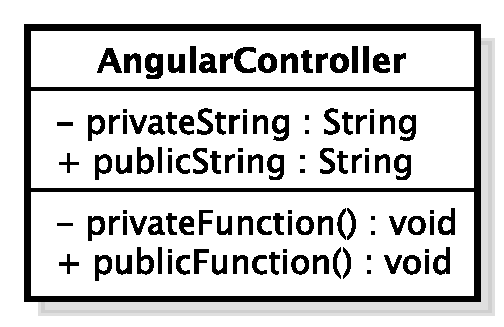
\includegraphics[width=3cm]{../immagini/angularController.pdf}
\caption{Esempio della definizione UML di un controller di Angular}
\label{fig:contorllerAngular}
\end{figure}
\FloatBarrier
\subsubsubsubsubsubsection{Directive}
Nelle descrizioni degli \textit{scope isolati} delle directive, la modalità con cui vengono passati i parametri utilizza la seguente notazione:
\begin{itemize}
\item \texttt{@:} indica che il parametro passato allo scope è una stringa e i cambiamenti effettuati su di essa dallo scope non sono visibili all'esterno;
\item \texttt{=:} indica che il parametro passato allo scope è un riferimento ad un oggetto;
\item \texttt{\&:} indica che il parametro passato è una funzione, che può avere dei parametri, e che lo scope può essere invocato dalla directive.
\end{itemize}
Come nome per l'oggetto \textit{scope} nella definizione di una directive si è scelto di utilizzare \texttt{scope} al posto di \texttt{\$scope} in quanto rispecchia il nome del campo dati utilizzato nella definizione della directive.\\
Nei diagrammi delle classi relative alle directive sono stati esplicitati solamente i campi dati, definiti da \gloxy{AngularJS}, necessari all'applicazione.
\subsubsubsubsubsubsection{Promise e \$q}
Tutti i metodi dei services che eseguono richieste al \gloxy{server} forniscono come valore di ritorno una promessa. Questo è stato modellato indicando come tipo di ritorno la classe \texttt{Promise}, maggiori informazioni riguardo l'interfaccia della classe e le \gloxy{API} offerte da \texttt{\$q} possono essere trovate nella pagina: \url{https://docs.angularjs.org/api/ng/service/$q}%$.
\subsubsubsubsubsubsection{Tipi di dato}
Per differenziare i vari tipi di dato usati forniti da \gloxy{Angular} si è scelto di utilizzare la seguente notazione:
\begin{itemize}
\item \texttt{Scope}: per i vari oggetti \texttt{\$scope};
\item \texttt{Promise}: per le promesse;
\item \texttt{DOMElement}: per gli oggetti jQuery o \gloxy{jqLite} passati alla funzione \texttt{link} di una directive;
\item \texttt{MouseEvent}: per gli oggetti jQuery che rappresentano un evento del \gloxy{browser} scatenato dal mouse dell'utente;
\item \texttt{\$nomeDelService}: per il tipo dei vari service, es: \texttt{\$http} indica il tipo del servizio \texttt{\$http}.
\end{itemize}
Maggiori informazioni riguardo le interfacce pubbliche di questi oggetti sono disponibili nella documentazione ufficiale dei \gloxy{framework}:
\begin{itemize}
\item \gloxy{AngularJS}: \url{https://docs.angularjs.org/api};
\item jQuery: \url{http://api.jquery.com}.
\end{itemize}
\subsubsubsubsubsection{Notazioni per il \gloxy{Back-End}}
Per convenzione i metodi definiti in questa componente non hanno mai tipo di ritorno. Infatti il tipo di ritorno in molti casi dipende dal comportamento \gloxy{runtime} del \gloxy{back-end}, questo può ritornare un messaggio d'errore oppure un oggetto Response contenente la risposta del \gloxy{server}.
\subsubsubsubsubsubsection{Express}
Nell'architettura definita dai \rPs si è preferito mantenere la notazione \texttt{nomeRouter} che veniva utilizzato nella versione 3 di Express, al posto di \texttt{nomeRoutes} della versione 4 di Express perché è stato ritenuto più significativo.
La motivazione di questa scelta deriva dal fatto che ogni modulo contiene tutte \textit{routes} logicamente correlate tra loro, è quindi più facile pensare ad un modulo come \textit{router} specifico anziché come un  aggregato di \textit{routes}.
Di conseguenza la cartella contenente i vari moduli di \textit{routes} si chiamerà \texttt{Routers} anziché \texttt{Routes}.
\subsubsubsubsubsubsection{\gloxy{MongoDB} e \gloxy{Mongoose}}
Come identificativo per la ricerca di oggetti nelle \texttt{collections} di \gloxy{MongoDB} vengono usati parametri di tipo \texttt{\gloxy{ObjectId}}. A livello di implementazione ai metodi con parametri di tipo \texttt{\gloxy{ObjectId}} verranno passate delle stringhe. La conversione viene effettuata automaticamente da \gloxy{Mongoose}.

\subsubsubsection{Codifica e convenzioni nei file}\label{codificaConvenzioniFile}
\begin{itemize}
\item Tutti i file devono essere conformi alla codifica \gloxy{UTF-8} senza \gloxy{BOM} (poiché potrebbe causare errori durante la procedura di verifica);
\item Per andare a capo viene usato il carattere LF (U+000A);
\item Modifiche alle convenzioni stabilite sono possibili solamente dopo una decisione del \rRP.
\end{itemize}
\subsubsubsection{Nomi e norme stilistiche nel codice}\label{normeStilisticheCodice}
\begin{itemize}
\item I nomi delle funzioni, delle variabili, dei metodi e delle classi devono essere scritti in lingua inglese;
\item I nomi delle classi devono avere la prima lettera maiuscola;
\item I nomi delle variabili, delle funzioni e dei metodi devono avere la prima lettera minuscola e le eventuali parole che ne compongono il nome devono avere la prima lettera maiuscola e non devono contenere underscore (es.: \textit{myFirstVar}, \textit{testFunction()});
\item Una funzione può avere al più 5 parametri;
\item Tutti i file \gloxy{JavaScript} devono essere salvati e consegnati come file con estensione .js;
\item Il codice \gloxy{JavaScript} non deve essere hard-coded all'interno del codice \gloxy{html} a meno che non sia inevitabile e quindi necessario;
%\item Gli script \gloxy{JavaScript} devono essere inclusi con: <script src= ``filename.js''>;
\item Questo tipo di tag devono essere posizionati il più avanti possibile nel codice \gloxy{html} in modo da ridurre gli effetti di ritardo imposti dal caricamento dello script all'interno della pagina;
\item Non c'è bisogno di utilizzare gli attributi \texttt{language} oppure \texttt{type}, infatti per lo standard \gloxy{HTML5} \gloxy{JavaScript} è riconosciuto come linguaggio di scripting di default;
\item Indentazione: l'unità di indentazione è 4 spazi, l'uso di tab deve essere evitato in quanto non esiste uno standard a riguardo, sarà quindi necessario utilizzare spazi anche se possono produrre file più pesanti, la differenza sarà praticamente nulla quando la versione del file da caricare verrà minificata;
\item Tutto il codice che deve essere eseguito sia sul \gloxy{client} sia sul \gloxy{server} sarà minificato;
\item Ogni linea di codice può essere lunga al più 80 caratteri, spezzarla nei punti dove si trovano gli operatori, o preferibilmente le virgole, per renderla più leggibile;
\item Tutte le variabili dovrebbero essere dichiarate prima di essere usate, permette di rendere il codice più leggibile e meno prono ad errori;
\item \`{E} vietato usare variabili globali implicite. In generale l'uso di variabili globali deve essere minimizzato il più possibile;
\item L'uso di funzioni globali deve essere per quanto possibile minimizzato;
\item Se si utilizzano variabili il primo statement nel corpo di una funzione deve essere \texttt{var}. In generale definire le variabili nella prima parte del corpo di una funzione;
\item Non devono esserci spazi tra nome della funzione e le parentesi () della lista dei suoi parametri;
\item Se si utilizzano funzioni anonime si deve inserire uno spazio tra la keyword function e le parentesi () della lista dei suoi parametri;
%\item Il simbolo ``\{'' deve essere allineato verticalmente rispetto al simbolo ``\}'' relativo;
%\item I costruttori devono essere scritti con il prefisso create, esempio createNomeCostruttore;
\item I nomi non possono contenere:
\begin{itemize}
\item Il carattere \$;
\item Il carattere backslash;
\end{itemize}
\item Le variabili globali vanno scritte a lettere maiuscole;
\item \`{E} vietato usare lo statement ``continue'';
\item In \gloxy{JavaScript} i blocchi non hanno uno scope. Solo le funzioni ed alcuni statement hanno uno scope. Non usare blocchi {} eccetto quando richiesto dal linguaggio.
\end{itemize}
\subsubsubsubsection{AngularJS}\label{normeAngular}
Per l'utilizzo di \gloxy{AngularJS} si è scelto di adottare le convezioni, suggerite dalla comunità di sviluppatori, reperibili al seguente indirizzo:
\begin{center}
\url{https://github.com/johnpapa/angular-styleguide}
\end{center}
Dovranno poi essere adottate le seguenti convenzioni:
\begin{itemize}
\item I costruttori dei \texttt{controllers} non sono soggetti a limitazioni sul numero di parametri;
\item I nomi delle \texttt{directives} dovranno avere il prefisso \texttt{premi};
\item Le \texttt{directives} dovranno avere sempre \texttt{scope} isolato, tranne in situazioni particolari, come nel caso di utilizzo di \gloxy{librerie} esterne. Scelte discostanti dalla normale prassi dovranno essere giustificate e sottoposte ad approvazione.
\end{itemize}
\subsubsubsubsection{\gloxy{MongoDB} e \gloxy{Mongoose}}
Per l'utilizzo di \gloxy{MongoDB} e \gloxy{Mongoose} si è scelto di adottare le seguenti convenzioni:
\begin{itemize}
\item Al posto dei costruttori vengono utilizzate funzioni statiche per avere un maggior controllo degli errori;
\item Come identificativo per cercare oggetti nelle \texttt{collections} di \gloxy{MongoDB} vengono usati parametri di tipo \texttt{\gloxy{ObjectId}}, anche se in realtà ai metodi vengono passate delle stringhe. La conversione viene effettuata automaticamente da \gloxy{Mongoose}.
\end{itemize}
\subsubsubsubsection{Commenti}
\begin{itemize}
\item L'utilizzo di commenti all'interno dei file contenenti codice è obbligatorio.
Ogni file deve iniziare con un'intestazione nella forma:\\
\textcolor{OliveGreen}{/**\\
**\\
** @class Nome della classe contenuta nel file \\
** @classdesc Descrizione della classe\\
** @author Autore del file (Indirizzo e-mail dell'autore)\\
** @description Data: data in cui è stato creato il file\\Requisiti: lista dei requisiti che il codice sorgente soddisfa \\
** @memberOf Nome del package che contiene la classe\\
**/}\\
\item Se nel file vi sono più funzioni o metodi va aggiunto un commento che specifichi una breve descrizione prima di ognuno di essi;
\item I commenti saranno scritti in lingua italiana;
\item I commenti presenti all'interno dei file di codice devono seguire JSDoc, le cui regole sono descritte all'indirizzo \url{http://en.wikipedia.org/wiki/JSDoc}.
\end{itemize}
\subsubsubsection{Ricorsione}
La ricorsione va evitata quando possibile. Per ogni funzione ricorsiva sarà necessario
fornire una prova di terminazione e sarà necessario valutare il costo in termini di occupazione
della memoria. Nel caso l'utilizzo di memoria risulti troppo elevato la ricorsione
verrà rimossa.
